
\subsection*{Practice taking Determinants}

%%%Insert this to get the typewriter font so it looks like a real movie script
{\ttfamily
\fontdimen2\font=0.4em
\fontdimen3\font=0.2em
\fontdimen4\font=0.1em
\fontdimen7\font=0.1em
\hyphenchar\font=`\-





%%%%put a hypertarget around the opening bit of text
\hypertarget{video_properties_of_determinant_practice}{Lets practice taking} determinants of $2 \times 2$ and $3\times 3$ matrices. 

For $2 \times 2$ matrices we have a formula
\[
\det
\begin{pmatrix}
a & b \\
c & d \\
\end{pmatrix}
= ad - bc\, .
\]
This formula might be easier to remember if you think about this picture.
\begin{center}
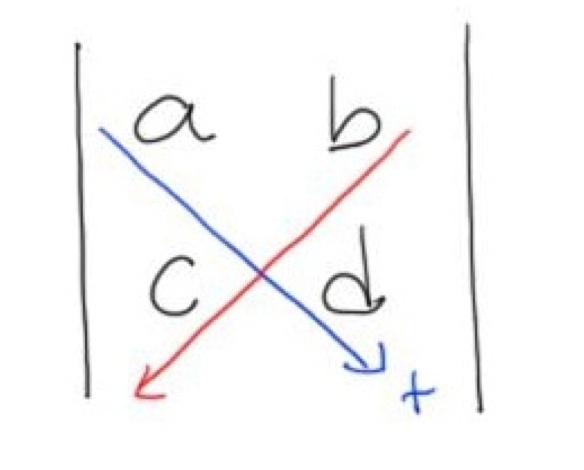
\includegraphics[scale=.20]{determinant_2by2.jpg}
\end{center}

Now we can look at three by three matrices and see a few ways to compute the determinant. We have a similar pattern for $3\times 3$ matrices. 
Consider the example 
\[
\det
\begin{pmatrix}
1 & 2 & 3 \\
3 & 1 & 2 \\
0 & 0 & 1 \\
\end{pmatrix}
= ( (1\cdot 1\cdot 1)+ (2\cdot 2\cdot 0) + (3\cdot 3\cdot 0)) - ((3\cdot 1\cdot 0)+ (1\cdot 2\cdot 0) + (3\cdot 2\cdot 1)) = -5
\]
We can draw a picture with similar diagonals to find the terms that will be positive and the terms that will be negative.

\begin{center}
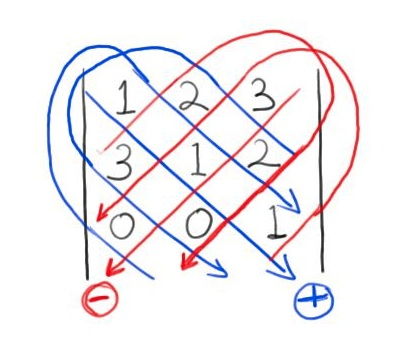
\includegraphics[scale=.35]{determinant_3by3.jpg}
\end{center}


Another way to compute the determinant of a matrix is to use this recursive formula. Here I take the coefficients of the first row and multiply them by the determinant of the minors and the cofactor. Then we can use the formula for a two by two determinant to compute the determinant of the minors%cite cofactor
\[
\text{det}
\begin{pmatrix}
1 & 2 & 3 \\
3 & 1 & 2 \\
0 & 0 & 1 \\
\end{pmatrix}
= 1 
\begin{vmatrix}
1 & 2 \\
0 &1\\
\end{vmatrix} 
-2 
\begin{vmatrix}
3 & 2 \\
0 & 1 \\
\end{vmatrix} 
+ 3 
\begin{vmatrix}
3 & 1 \\
0 & 0 \\
\end{vmatrix}\\
 = 1(1-0) - 2(3-0) + 3(0-0) = -5
\]
Decide which way you prefer and get good at taking determinants, you'll need to compute them in a lot of problems.
%%%%don't forget to close the bracket so the stuff after your file doesn't look like a movie!
}

%\newpage
